\documentclass{article}
\usepackage[utf8]{inputenc}
\usepackage{multirow}
\usepackage{verbatim}
\usepackage[pdftex]{graphicx}
\usepackage{subfigure}


\begin{document}
\title{Profiling users media preferences based on social network data streams}
\author{Konrad Delong \and Antoni Piechnik}
\date{May 25 2010}

\maketitle

\begin{abstract} Social networks have been becoming hugely popular over the last
years. With enormous number of people sharing information about their lives,
they are now a great source of information about their interests. Based on both
structured data (such as the social aspect of YouTube) as well as unstructured
(Twitter), we will be trying to find out how accurately we can profile user's
preferences for it to be usable in a real life project (NoTube).
\end{abstract}

\section{Introduction}

Recommender systems used to involve recommending more physical objects \cite{combining-cf-with-pa} to users.
However, more and more abstract topics are becoming parts of such recommenders (such as tags) \cite{accuracy-recommending}. The NoTube project bases its recommendation of TV programmes on aggregating,
extracting and analyzing user activities \cite{notube-main}.

On the Web, a great deal of \textit{user activity data} can be found on several networks. This UAD (\textit{user activity data}) varies from user video viewing history and subscriptions to video channels (\eg \textit{YouTube}) to users' activity updates formed in natural language (such as \textit{Twitter}) \cite{why-we-twitter}.

In this paper we experiment on those data streams and evaluate their usefulness to the user profile generation. We answer
two main research questions:
\begin{enumerate}
  \item What user data can we collect from \textit{structured} and \textit{unstructured} user activity streams?
  \item How useful is \textit{structured} UAD as compared to \textit{unstructured} UAD, to generate a user profile?
\end{enumerate}

By the \textit{structured} user activity data, we understand data organized in predefined
preference groups (such as favorites, subscriptions, etc. on \textit{YouTube}).
We define \textit{unstructured} UAD, on the other hand, as data formed in freely in
natural language (user streams on \textit{Twitter}).

To answer the first research question, we mainly focus on analyzing the available
data and the way people use services such as \textit{YouTube} and \textit{Twitter} to share
their media preferences.

We answer the second research question by presenting methods for evaluating results of
available data aggregation and user profiling for both services with a comparative analysis.
Our research reveals that more complex methods are required when processing \textit{unstructured} UAD.
We have also observed that there are differences in the amount of user profiling data as well as its
accuracy. However, despite those differences, both of them may provide
enough opportunities for user media preference extraction.

In the following section we describe related work on the subject. In section 3, we describe
a selection of sources of user activities on the Social Web. Section 4 contains the description of
the vocabulary we employed in our experiments. We follow by detailing the results of our experiments
with the usage of \textit{structured} (section 5) and \textit{unstructured} (section 6) user activity data.
The next part of the paper (section 7) is a comparison of the usage of both kinds of UAD. Section 8
details the user evaluation of generated profiles. We conclude with a section on future
work, a summary (section 9) and our implementation details (section 10).

\section{Related work}

A considerable number of papers examining social Web services have been
published. Works devoted to YouTube often contain analysis of the video data
stored by the service and its implications to the traffic generated
(\cite{i-tube-you-tube}, \cite{views-from-the-edge},
\cite{statistics-and-social-network}), some study impact of YouTube service on
very narrow topics, like 2006 USA presidential elections
\cite{voters-myspace-youtube}, or social attitude towards vaccinacions
\cite{keelan}. There are also papers analyzing privacy issues of using YouTube
\cite{publicly-private}.

Works analyzing \textit{Twitter} as a data stream can differ from very general \cite{why-we-twitter},
to works devoted to analyzing content of the \textit{Twitter} users' timelines (such as \cite{twitter-content-is-it} and \cite{short-tweet}).

There are also works devoted to automated user profile generation, covering multiple data sources for profile
information aggregation \cite{public-profiles}, as well as abusing social networks for profile generation \cite{twitter-abuse}. Apart from profile generation, a URL recommender system for \textit{Twitter} users
has been introduced by \cite{short-tweet}.

The works describing user profiling in general are focused on finding the basic user profile ontology \cite{creating-ontology-for-user-profile}, and their role in recommender systems area \cite{ontological-user-profiling}.

Apart from the papers mentioned, we have also found various implementations of systems that aggregate personal preferences based on different
social services:

\paragraph{Hunch}
\textit{Hunch}\footnote{http://www.hunch.com} is a service offering recommendations on different topics based on a user's \textit{Twitter} data. It predicts preferences in forms of small questions and is then able to recommend a product or a solution to a problem that is represented with a \textit{Topic} on the site. \textit{Hunch} seems to be more commercial-oriented, \eg providing users with links to online stores with products they are recommending. However,
it's prediction results suggest that \textit{Twitter} users' timelines contain information about their preferences.

The application can create recommendations based solely on user's \textit{Twitter} data (mostly people they follow). However, when little data is available, it requires input from users in order to make future predictions more accurate. It covers topics broader than the \textit{NoTube} project.
\textit{Hunch.com} does not provide information on how the recommender system works, although it provides an API for accessing their data.
Hunch is able to adapt to much more different topics, and it does not necessarily focus on their semantics (rather on what similar people simply like).


\section{User activity data on the Social Web} 
\label{sec:uad}
In order to answer the first research question, we have focused on data from two social services: \textit{YouTube} and
\textit{Twitter}. The goal of this chapter is to present the organization of the \textit{user activity data} (UAD)
available in those two networks.

In the section \ref{sec:youtube_uad} we describe user data available via APIs for
\textit{YouTube}, whereas section \ref{sec:twitter_uad} covers possible methods of extracting preference information
from \textit{Twitter} users' tweets. We will use the expression \textit{named entity} (NE) to refer to
known media people, shows and programs. The NE data has been collected from the \textit{Freebase} dataset,
which we described in section \ref{sec:vocabulary}.

\subsection{YouTube}
\label{sec:youtube_uad}

\textit{YouTube} stores various data concerning its users and content and offers a public
access to this structured information through the use of its API. In theory, additional
pieces of data could be acquired through the use of screen scraping. Using this
technique, however, breaks \textit{YouTube}'s Terms and Conditions (\S 5.1H), and as such
was not used for this research.

The schema of \textit{YouTube} data is presented in tables 1-5.  Each table lists
properties of a single type of entity, along with the way those properties are
accessed (either API or through the use of screen scraping). For example:
we can learn that values of such video's parameters as its view count or
its duration (and many others) are accessible through the official API.

Among these elements, what begs for most attention are the video sets.
Undoubtedly, videos are the central point of \textit{YouTube} as a service, and form the
majority of its content. This sets them as most suitable candidates for data
enrichment. Furthermore, the user can form a relation with a video by performing
an action on it (uploading, adding to favourites or subscribing), which makes
video analysis a perfect choice for semantic user profile generation.  Three
sets of videos are accessible through the official API, these are
\emph{favorites}, \emph{subscriptions} and \emph{uploads}. For this reason, the
rest of \textit{YouTube} research in this paper will focus on these three sets. The other
fields concerning user, like his \textit{age} or \textit{location}, while
directly usable as a part of the profile, are not as challenging to extract and
will not be analyzed in deep detail. \textit{YouTube} also contains demographic data
of a user, which we will not use in our experiments.

\begin{center}
  \begin{tabular}{|p{3cm} | l | p{4cm}|} \hline
  Information & Access & Notes\\ \hline
  Title & Public API & Natural language \\
  Published & Public API & \\
  Updated & Public API & Date \\
  Category & Public API & Chosen from a restricted set of YouTube categories \\
  Tags (keywords) & Public API & May be freely assigned \\
  Comments & Public API & Natural language \\
  Permissons & Public API & Irrelevant, but available \\
  Description & Public API & Natural language \\
  Thumbnails & Public API & Set of video's thumbnails (along with times
  when taken) \\
  Duration & Public API & \\
  Ratings & Public API & Best, worst and average rating, number of votes \\
  Viewcount & Public API & \\
  Favourite count & Public API & \\
  Number of likes & Public API & \\
  Number of dislikes & Public API & \\
  Aspect ratio & Public API & \\
  Related & Public API & \\
  Responses & Public API & \\
  Author & Public API & \\ \hline
  \end{tabular} \\
  Table 1: Information available for a video \\
\end{center}

\begin{table}[htb]
	\begin{minipage}[b]{0.5\linewidth}
	\centering
		\begin{tabular}{ | p{3cm} | l |}\hline
		Information & Access \\ \hline
		Number of results & Public API \\
		Search results & Public API \\ \hline
		\end{tabular}
		Table 2: Information available for video search results \\

		\begin{tabular}{ | p{3cm} | l |}\hline
			Information & Access \\ \hline
			Created & Public API \\
			Updated & Public API \\
			Author & Public API \\
			Text & Public API \\ \hline
		\end{tabular}
		Table 3: Information available for a comment \\

		\begin{tabular}{ | p{3cm} | l |}\hline
			Information & Access \\ \hline
			Demographics & Screen scraping \\
			Referrers & Screen scraping \\
			Countries popularity & Screen scraping \\ \hline
		\end{tabular}
		Table 4: Information available for a channel \\
	\end{minipage}
	\hspace{0.5cm} % no new lines here!!
	\begin{minipage}[b]{0.5\linewidth}
		\centering
		\begin{tabular}{ | p{3cm} | l |}\hline
			Information & Access\\ \hline
			\emph{Uploads} & Public API \\
			Gender & Public API \\
			Location & Public API \\
			Age & Public API \\
			Contacts & Public API \\
			Username & Public API \\
			\emph{Subscriptions} & Public API \\
			Inbox & Public API \\
			\emph{Favorites} & Public API \\
			History & Screen scraping \\
			Likes & Screen scraping \\
			Issued authentication subtokens & Screen scraping \\ \hline
		\end{tabular}
		Table 5: Information available for a user
		\label{ut_user_info}
	\end{minipage}
\end{table}

\subsubsection{Problems regarding concepts identification}

Even though the video sets are most promising mean to interest extraction. There
are problems that make this task challenging.

\paragraph{Detecting level of interest}
One of them, is the fact that YouTube videos cannot
express an interest directly. The user can add a video to the favourites
indicating some level of interest, but we are not able to detect the reason for
such user's action. This indirectness might result in lower precision of the
interests extracted from YouTube. 

The only indicator of an interest in a particular subject is binary: it is
either present or not present in user's data. This forces us to fall back to
entity counting in order to determine level of interest.

\paragraph{Usage of YouTube features} 
Another problem is the scarcity of data. Below are measurements that showed how
little users make extensive use of YouTube features.
In order to find out how frequently the mentioned sets are used, a sample of 7,500
randomly chosen users was examined. Among those users, noticeable differences in their
activity (level of use of various features) were noted. Many users show little activity,
as compared to a few highly active users.  50\% analyzed accounts had less than 60 favourites,
6000 out of 7,500 had less than 40 uploads.  All histograms on Figure 1 show
numbers of users (axis y) with $x_1-x_3$ numbers of
favourites/subscriptions/uploads. For all three cases, almost all users belonged
to the first histogram range -- the one with least items. As number of items
grows, the number of users decreases so quickly, that logarithmic scale has been
used in order to increase the readability of the charts.

For all three sets, almost half of examined users had no more than 100 items.
This means that for most cases, the user profiling would need to be based on
little amount of data.

\begin{figure}[htb]
  \centering
  \subfigure[Favourites]{
		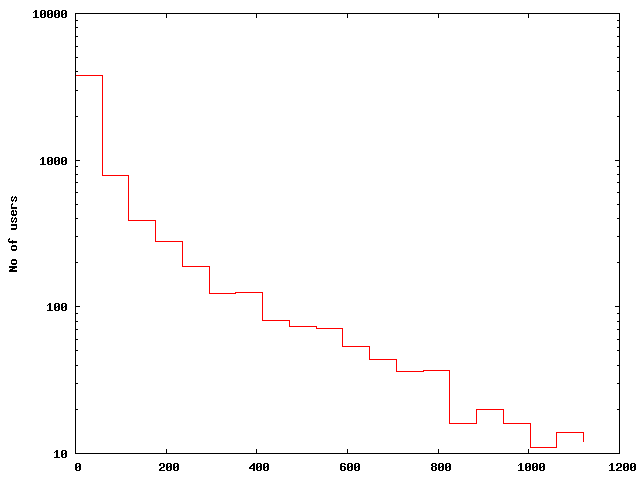
\includegraphics[scale=0.6]{images/favs.png}
		\label{fig:favs}
  }
  \subfigure[Subscriptions]{
		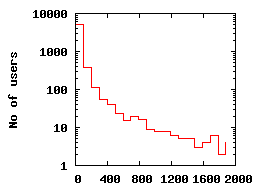
\includegraphics[scale=0.6]{images/subs.png}
		\label{fig:subs}
  }
  \subfigure[Uploads]{
		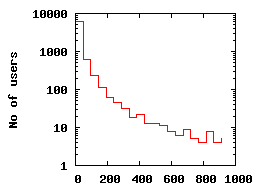
\includegraphics[scale=0.6]{images/ups.png}
		\label{fig:ups}
  }
  \label{fig:subfigureExample}
  \caption{Histograms of usage of favourites \subref{fig:favs}, subscriptions
  \subref{fig:subs} and uploads \subref{fig:ups}. The x axis represents groups of
  users having $x_1-x_2$ entities, the height of the bars indicates sizes of the
  groups.}
\end{figure}

\subsubsection{YouTube measurements employed}

We have decided to measure the user data in two ways: by identifying entities
and collecting tags. Each YouTube video contains a set of tags - single,
separate words - describing the video's content. While this kind of information
is not directly usable for the recommender systems, it can prove indirect
support for verifying the hypothesis that recommenders prepared. The types of
measurements performed are presented in Table 6.

\begin{center}
  \begin{tabular}{ | p{4cm} | p{7cm} | } \hline
    \multicolumn{2}{|c|}{Types of measurements available} \\
    \hline
    \multirow{3}{*} {Tag collection}
      & Tags from favourites \\ \cline{2-2}
      & Tags from subscriptions \\ \cline{2-2}
      & Tags from uploads \\ \cline{2-2}
    \hline
    \multirow{3}{*}{Concepts detection}
      & Concepts from favourites \\ \cline{2-2}
      & Concepts from subscriptions \\ \cline{2-2}
      & Concepts from uploads \\ \cline{2-2}
    \hline
  \end{tabular}
Table 6: Overview of the measures available for the \textit{YouTube} structured data \\
\end{center}

\subsubsection{YouTube video descriptions corpus}

A corpus of titles and descriptions for little over 100,000 videos was collected
for text-based analysis of YouTube data. The file's size was 36 Mbytes. This
data was used to compute number of video descriptions with identifiable concepts from
\textit{Freebase}\footnote{http://freebase.com} data vocabularies (more on this in section 4).

\subsection{Twitter}
\label{sec:twitter_uad}

Data available on \textit{Twitter} is composed of natural language short messages posted by users
consisting of up to 140 characters, commonly known as \textbf{tweets}. Within
those tweets we can distinguish user mentions (\textit{Twitter} usernames preceeded with the symbol @,
such as \textit{@justinbieber}\footnote{http://twitter.com/justinbieber}) as well as topics in form of
\textit{hashtags} -- names stripped of all whitespace and preceded by the hash symbol,
\eg \textit{\#TheDailyShow} \cite{edinburg-corpus}.

The initial purpose of tweets was to inform other users of currently performed activities. However, as this service has
evolved, users started to use \textit{tweets} for a variety of purposes, such as conversations,
sharing information/URLs and reporting news \cite{why-we-twitter, twitter-content-is-it}. In this section we describe available methods to use such unstructured data.
In our experiments we focus on the following NE extraction methods:

\paragraph{Mentioning NE full names}
Using simple string matching methods, we search for NE labels within tweets.
Occurrences of NE names in tweets indicate a potential interest in the NE mentioned. The
number of references is expected to be positively correlated with the level of interest in the given NE \cite{twitter-content-is-it}.
Entities might be mentioned by:
\begin{itemize}
  \item \textit{full name} (\eg \textit{"Having a How I Met Your Mother marathon."})
  \item \textit{hashtag} (\eg \textit{"Who?! Where? I love \#HowIMetYourMother!"})
  \item \textit{twitter username} (NE's twitter username, if known, \eg \textit{"@HIMYM\_CBS It entertains the spirit"})
  \item \textit{acronyms} (\eg \textit{"Watching HIMYM. Season 3."})
\end{itemize}
\paragraph{Usage of opinion vocabulary when tweeting about NEs}
In order to extract opinion towards a NE from a tweet, vocabularies that express
opinion has been compiled. They have been pragmatically chosen by looking at random tweets.
This vocabulary contains the following words: \textit{awesome, bad, enjoyed, good, great, hate,
like, liked, love, loving, poor, recommend, stunning, worst}.
Those verbs were searched for in the tweets containing NE mentions.
Example of a tweet: \textit{"yesterday's \#Lost episode was stunning!"}
\paragraph{Usage of activity verbs when tweeting about NEs}
When mentioning a media-related NE, users may also describe the activity performed.
In order to find such tweets, an activity verbs vocabulary has been prepared (similarly to
the opinion verbs, it was chosen by looking at the contents of random tweets).
This vocabulary contains the followings verbs: \textit{watching, watched, play,
watch, playing, saw, seen, played}.
Describing the activity of participating in a certain TV experience, such
as watching a show, has to be noted due to the fact that Twitter users are more
likely to specify what they are doing at a particular moment.
Example of a tweet: \textit{"Finnally watched Ironman 2 aha'"}

\paragraph{Extracting NEs from structured twitter stream sources}
Applications, such as \textit{YouTube} or \textit{Boxee}\footnote{http://www.boxee.tv}, automatically generate tweets
if the user linked their Twitter account with that application. These tweets are
usually well structured, and therefore very suitable to extract a NE, activity or preference.
Examples of tweets: (\textit{Boxee}) -- \textit{"likes Inglourious Basterds on Boxee http://bit.ly/FbAbn"} and
\textit{YouTube} -- \textit{"I liked a YouTube video -- How I Met Your Mother - Lorenzo Van Matterhorn"}

\paragraph{Summary}
We present the possible measurements for extracting the UAD from
\textit{Twitter} in Table 7:

\begin{center}
  \begin{tabular}{ | p{4cm} | p{7cm} | } \hline
    \multicolumn{2}{|c|}{Types of measurements available} \\
    \hline
    \multirow{4}{*} {Mentioning NEs}
      & Full name matching \\ \cline{2-2}
      & Matching the twitter username (if known) \\ \cline{2-2}
      & Matching name converted to a hashtag form \\ \cline{2-2}
      & Matching the full name acronym \\ \cline{2-2}
    \hline
    Usage of activity verbs & Mentions using activity verbs \\
    \hline
    \multirow{3}{*}{Using preference verbs}
      & Mentions using preference verbs \\ \cline{2-2}
      & Positive preferences \\ \cline{2-2}
      & Negative preferences \\ \cline{2-2}
    \hline
  \end{tabular}
Table 7: Overview of the measures available for the \textit{Twitter} UAD extraction \\
\end{center}

\subsubsection{Corpus used for research}

The example data analyzed consists of 43,000 tweets of 203 different users.
They have been selected by looking at the followers of popular TV channels and broadcasters
available on Twitter. Users were selected based on the number of tweets and their followers.
For our experiments, we have focused on tweets in English.

The most significant reason for using a precompiled corpus for this research is the Twitter API
Rate Limiting which limits the amount of tweets that can be fetched using the API.
Furthermore, a great deal of Twitter users provide data not necessarily
useful for our experiments. Mentions of NEs in non-English tweets could be located, but
extracting preference information in a multi-lingual setting is more challenging.
Using a preselected corpus enables measuring and comparing the effectiveness of different
counting methods much easier \cite{short-tweet}.

\subsection{Metrics used in constructing User Profile}

The generated user profile is a collection of concepts along with their
weights. In order to keep the scale of the weight simple (more on that in section
\ref{sec:evaluation}), we limited the scale to an integer range from 0
up to 3, meaning accordingly: ''do not like'', ''neutral'', ''like'', ''like
very much''. In order to determine the weight for each concepts, simple metrics
were used: number of repeats normalized to the mostly repeated item for
YouTube, and type of mention, the amount of mentions of a specified NE as well
activity/preference vocabulary usage for Twitter.



\section{Extracting user profile from Twitter}

In this section, we will evaluate the use of entity reference extractions
mentioned in Section 3.2 when ran against the \textit{Twitter} corpus (as described in Section 3.2.1).
We will discuss the results and their usefulness for generating a media preference profile of a user.
We will also cover any problems encountered and suggest possible solutions.

\subsection{Approach}
Since the \textit{Twitter} corpus has been selected as described in the Section 3.2.1,
we decided to cross-validate the measurements against two randomly selected halves of the corpus
to be able to minimize the overfitting of the data. By measurements, we understand methods of
entity reference extraction described in Section 3.2.

We have used vocabularies consisting of \textit{TV Actors, TV Programmes, Movies and Movie Actors} from
the \textit{Freebase} dataset.

Initial results show that using simple string matching methods we are able to extract interests from
a user's Twitter stream. For an active Twitter user, it holds that on average up to \textit{18\%} of their tweets
contain mentions of media entities (more on that in section 8.2).

However, there is a great number of entity names (mostly TV Shows) that create noise in the results, \eg show titles such as \textit{Me too}. Removing those false positives has a crucial effect on the eventual accuracy of a Twitter-based profiler
(as we shall see in section 8.3.1).

\subsection{Results}
In this section we present results of locating references to entities using different methods (as described in Section 3.2).
In each paragraph we present results for both halves of the corpus, which we will refer to as \textit{Corpus 1} and
\textit{Corpus 2}.

\subsubsection{Detecting mentioned entities}
\paragraph{Full name matching}
We have measured the average ratio of tweets with entities found to all tweets for different kinds of entities using full name matching of the entity name.

\begin{center}
  \begin{tabular}{ | p{4cm} | p{2cm} | p{1cm}| p{2cm} | } \hline
    Entity (average) & Corpus 1 & & Corpus 2 \\ \hline
    TV Shows & 1.24\% & & 1.76\% \\ \hline
    TV Actors & 0.41\% & & 0.00\% \\ \hline
    Movies & 1.92\% & & 1.69\% \\ \hline
    Movie actors & 0.74\% & & 0.21\% \\ \hline
  \end{tabular} \\
  Table 8: Percentage of all tweets with recognized entities using full name matching \\
\end{center}

Scores presented in Table 8 are used as the a baseline below. Out of half of the corpus, an average of 224 tweets contained reference for each entity type (898 tweets in total). This is a low score, but considering the purpose of \textit{Twitter} (as described in section 3.2), we have been expecting them and still believe this amount might be enough for user profiling.

\paragraph{Matching twitter usernames}
Due to small number of available Twitter usernames for entities in the \textit{Freebase} dataset (as of writing this paper -- 182 \textit{Twitter} usernames related to TV), this approach is not proving effective. After including those usernames in the search,
we noticed little (0.02\% in on of the corpuses for TV Shows) to almost none increase in the results.

\paragraph{Matching title acronyms}
Only entities with a title of 3 or more words have been used for this measurement, since searching
for smaller acronyms has generated a great amount of noise in the results. We have omitted Actors names, because
they mostly consist of two words and their acronyms rarely correspond to those actors.

\begin{center}
  \begin{tabular}{ | p{4cm} | p{2cm} | p{1cm}| p{2cm} | } \hline
    Entity (average) & Corpus 1 & & Corpus 2 \\ \hline
    TV Shows & 3.07\% & & 2.17\% \\ \hline
    Movies & 2.01\% & & 2.33\% \\ \hline
  \end{tabular} \\
  Table 8: Percentage of all tweets with recognized entities using the entity's name acronym \\
\end{center}

We can easily spot an increase in matched entities, since acronyms such as \textit{SNL}
(for \textit{Saturday Night Live} show) or \textit{BBT} (\textit{Big Bang Theory}) are widely used.
However there might be many misleading acronyms created with this approach. If an acronym is similar
to a natural language word (\eg \textit{CAT}), it will drastically increase the noise and the amount
of \textit{false positives} generated by the matching algorithms (thus the higher percentage of tweets
found). This problem might be solved by methods for avoiding the false positives, which we discuss in section 6.3.

\paragraph{Matching of the name converted to a hashtag form}
For this measurement, all entities' names have been converted to a \textit{hashtag} form (as described
in Section 3.2). In this experiment, also one-word entity names have been used.

\begin{center}
  \begin{tabular}{ | p{4cm} | p{2cm} | p{1cm}| p{2cm} | } \hline
    Entity (average) & Corpus 1 & & Corpus 2 \\ \hline
    TV Shows & 1.18\% & & 2.21 \% \\ \hline
    TV Actors & 0.00\% & & 0.03\% \\ \hline
    Movies & 2.49\% & & 3.12\% \\ \hline
    Movie actors & 0.67\% & & 0.09\% \\ \hline
  \end{tabular} \\
  Table 10: Percentage of all tweets with recognized entities using hashtag formed from the entity name \\
\end{center}

The results in Table 10 let us notice how the person-based entities have either noted a smaller
occurrence rate and the title-based ones have improved. This may be related to the
fact that people usually create hashtags based on a more general entity (such as
a movie) rather then it's specific parts (such as actors that play in it)
when expressing their opinion \cite{edinburg-corpus}

\subsubsection{Detecting opinion on an entity}
\paragraph{Usage of activity verbs}
For this experiment, a rather small activity verbs vocabulary has been used. (verbs such
as \textit{to watch, to play, to see, to check out, to catch} with their past forms.
\\ Below is a figure showing percentage of tweets using an activity verb
and a entity name (full match) out of all that have been matched with an
entity's name (hence the higher scores).

\begin{center}
  \begin{tabular}{ | p{4cm} | p{2cm} | p{1cm}| p{2cm} | } \hline
    Entity (average) & Corpus 1 & & Corpus 2 \\ \hline
    Movies & 37.4\% & & 24.3\% \\ \hline
    TV Shows & 21.2\% & & 13.4\% \\ \hline
    TV Actors & 1.3\% & & 0.6\% \\ \hline
    Movie actors & 2.1\% & & 0.0\% \\ \hline
  \end{tabular} \\
  Table 11: Average ratio of tweets with activity verbs found to all tweets with entity references. \\
\end{center}

As we can see, the activity verbs are very unlikely to be occurring next to
person-based entities. However, activity verbs are much more popular with both
Movies and TV Shows, which originates from the very idea of Twitter for
updating statuses with information on what the user is currently doing (such as \textit{watching}
a movie).

\paragraph{Usage of preference vocabulary}
Two sets of preference have been used:
\begin{itemize}
  \item positive -- such as \textit{like, recommend, love, great, awesome, stunning, good}
  \item negative -- such as \textit{hate, bad, worse, poor}
\end{itemize}

The Table 12 below shows the general use of preference verbs with occurrences of
mentions.

\begin{center}
  \begin{tabular}{ | p{4cm} | p{2cm} | p{1cm}| p{2cm} | } \hline
    Entity (average) & Corpus 1 & & Corpus 2 \\ \hline
    TV Shows & 7.4\% & & 6.3\% \\ \hline
    Movies & 9.1\% & & 8.4\% \\ \hline
    TV Actors & 0.0\% & & 0.9\% \\ \hline
    Movie actors & 1.2\% & & 2.7\% \\ \hline
  \end{tabular} \\
  Table 12: Average ratio of tweets with preference verbs found to all tweets with entity references \\
\end{center}

We have also measured the positive-to-negative preference ratio (Table 13):

\begin{center}
  \begin{tabular}{ | p{3cm}| p{2cm} | } \hline
    Type & Amount \\ \hline
    Positive & 92\% \\ \hline
    Negative & 8\% \\ \hline
  \end{tabular} \\
  Table 13: The amount of positive and negative verbs found within the tweets with entity references found \\
\end{center}

The amount of preference verbs used whilst mentioning an entity is definitely
smaller compared to activity verbs. However, the positive-to-negative ratio suggests that users'
media preferences expressed on Twitter are mostly positive.

\paragraph{Preference towards entities followed by a user}
By gathering available Twitter usernames from the \textit{Freebase} database,
we were able to perform searches for mentions of those usernames within the followers' streams.

The Table 14 shows the share of different kind of mentions of the specific entity while following.

\begin{center}
  \begin{tabular}{ | p{3cm}| p{2cm} | } \hline
    Match type & Occurence \\ \hline
    Name & 0\% \\ \hline
    Hashtag & 8\% (2 occurrences) \\ \hline
    Username & 92\% (22 occurences) \\ \hline
  \end{tabular} \\
  Table 14: The amount of mentions by different methods of the entity being followed by a user in his stream \\
\end{center}

Since Twitter usernames mostly represent specific people rather than any other kinds of entities, it seems as if users mostly
mention them using their usernames rather than their names in plain or hashtag form.

However, those mentions occur relatively rarely. For a sample of 70 twitter usernames and 5 followers each
(around 4000 tweets), we were able to find out only 24 tweets (about 0.57\%) mentioning directly the people they are following.

Furthermore, following a certain entity should also be regarded just as a preference toward the topics this entity is related to (such as Politics for \textit{BarackObama}). On the other hand, automated locating of more \textit{official} twitter usernames for various entities is challenging, which
limits the use of this approach.

\subsection{Avoiding false positives}
By \textit{false positives}, we understand matches that have been falsely assigned to a user stating user's interest.
They occur usually when a user uses the entity name in a unrelated context when the entity name is similar to a
part of natural language.

In order to reduce the chance of such accidental name matches occurring, entity names were ran against a corpus
of English texts, ranking them by their frequency. The more often an entity name occurs in those corpora, the smaller the chance of it occurring as a name of the TV shows rather than a natural language expression. In order to rate the certainty, a separate function is introduced, taking into account the following:

\begin{itemize}
  \item form of occurrence of the entity name (string match, hashtag)
  \item use of an activity verb
  \item use of a preference verb
  \item the frequency of the entity name in a collection of samples of written and spoken language
\end{itemize}

We expect the first three of those factors to have a huge influence on the accuracy of the entity recognition within a tweet (basing on results in section 6.2). The can see in section 8.3.1 that such approach provided great results for
reducing the amount of false positives.

This measurement is easily translatable into the preference weights to be recorded when profiling a user.
Moreover, by undertaking semantic approaches we are able to analyze different topics found in a tweet and
attempt to rank their relation to the entity we are researching. We will discuss this in the section 9 (Future work).



\section{Using structured user activity data from YouTube}

Our goal is to extract a user profile. For this paper, we will assume that user
profile is a collection of linked data concepts and weights, that should be understood as
user's interests. Many YouTube videos have semantic meaning -- they can
be associated with existing concepts (like actors or music bands) by performing
text search. In addition to that, analysis of tags can give an overview of user's
interests. This kind of data is useful in two
ways: first, it lets easily identify interests for a user, second: it can be
used to verify interests generated with other methods..

In the following sections, we will describe methods used to generate the user
profile. First, we describe our tag counting approach and compare the possible
use of tags and categories in user profiling. Then we will discuss possible
additional information coming from repeating occurrences of the tags in
different sets of videos. The next subsection present the double
nestedness problem, which makes counting tags from subscriptions fundamentally
different that the other two sets. The last subsection describes matching
YouTube videos to actual linked data concepts.

\subsection{Counting YouTube tags and categories}
Analyzing tags information carries some problems. Tags of a single video clip
can be either too numerous, making many
of them irrelevant, too sparse, nonexistent and occasionally just wrong. To avoid
that problem, we aggregate the tags across sets of video clips related to the
profiled user (favourites, subscriptions, uploads). Similar aggregation was
performed for the videos' categories. Below is a comparison of results of counting
tags (chosen by the user) and categories (picked from a small predefined set).


\begin{table}[ht]
\begin{minipage}[b]{0.5\linewidth}\centering

\begin{tabular}{| l | l |}
Category & \# \\ \hline
News & 8 \\
Music & 5 \\
Education & 3 \\
Comedy & 2 \\
\end{tabular}

\end{minipage}
\hspace{0.5cm}
\begin{minipage}[b]{0.5\linewidth}
\centering

\begin{tabular}{| l | l |}
Tag & \# \\ \hline
sonik & 5 \\
bogusław & 5 \\
trzech & 5 \\
kupli & 5 \\
wybory & 4 \\
kraków & 4 \\
polska & 4 \\
\end{tabular}

\end{minipage}

\caption{Most popular tags and categories from account of Bogusław Sonik -- a
polish politician. The word ''wybory'' stands for ''election'' in polish, and
\emph{Trzech kumpli} is a title of a controversial political documentary.}
\end{table}


\begin{table}[ht]
\begin{minipage}[b]{0.5\linewidth}\centering

\begin{tabular}{| l | l |}
Category & \# \\ \hline
Music & 53 \\
Comedy & 20 \\
Entertainment & 8 \\
Games & 4 \\
People & 3 \\
Travel & 3 \\
News & 2 \\
\end{tabular}

\end{minipage}
\hspace{0.5cm}
\begin{minipage}[b]{0.5\linewidth}
\centering

\begin{tabular}{| l | l |}
Tag & \# \\ \hline
metal & 17 \\
music & 11 \\
rock & 11 \\
video & 7 \\
the & 7 \\
black & 7 \\
of & 7 \\
\end{tabular}

\end{minipage}

\caption{Most popular tags and categories from anonymous user -- apparently a
heavy metal music fan}
\end{table}

We can see that category count, even though providing general overview of
person's interests (and the ways she uses youtube), cannot be used to find
specific interests. We can say that a person is more keen to
favourite music videos or comedy videos after looking at his categories, but in
order to say what kind of music the person prefers, we need more specific
information gathered from \eg tags.

\subsection{How to handle duplicates}

When combining tags collected from various sets of videos, a question should be
asked what preference -- if any -- should be given to tags appearing in more
then one of them. Let's analyze some examples. The letters $f$, $s$ and $u$ mean number
of videos in accordingly: favourites, subscriptions and uploads. The
combinations of letters indicate the size of the intersections of those sets. \\

\begin{tabular}{| l | l | l | l | l | l | l | l |}
user & $f$ & $s$ & $u$ & $fs$ & $fu$ & $su$ & $fsu$ \\ \hline
politician & 219 & 32321 & 357 & 116 & 59 & 156 & 34 \\
metal music fan & 1103 & 7570 & 73 & 533 & 27 & 44 & 26 \\
one of authors & 687 & 5553 & 10 & 199 & 2 & 2 & 1 \\
\end{tabular} \\

The tags that appeared in all three sets are:
\begin{itemize}
  \item{politician: \emph{wybory, europarlament, czerwca, europa, europejska,
  parlament, 18, unia, europejski, kraków, w, 7, pe, 2009, bogusław, po,
  bezpieczeństwo}}
  \item{metal music fan: \emph{head, death, pantera, for, in, nosturi, the, live, cover, metal}}
  \item{one of authors: \emph{film}}
\end{itemize}

As expected, the tags in the intersection of sets give much more precise view of person's
interests as compared to tags occurring in a single set. Tags get muted when a user is not active in one of
those areas (\eg does not upload movies very frequently). In order to minimize it's effect on the
end result, weights for different sets may be used, and we can maximize weights for tags occurring
in multiple sets.

\subsection{The double nestedness problem}
Gathering tags across user's favourites or uploads let us treat the whole video
set as a single document, giving each tag equal weight in the counting process.
Taking a similar approach for subscriptions (\eg giving equal weight to each
tag of each video of every subscription) leads to some unwanted effects.

Suppose a user subscribes to two channels. One represents the british royal
family (133 uploads), the other one: Apple Inc., an american computer company
(19 uploads). The tags referring to new hardware releases would get flooded with
tags regarding british-specific content. In effect, the user's profile would
depend on third parties' youtube activity which is doubtful to be of any
importance to her.

In order to counteract this effect a number of techniques can be used. One of
them is giving tags in each subscription a weight, based on the number of videos or
total number of tags.

\subsection{Identifying entities in Youtube streams}
The linked data concepts can be associated with user data through the use of
simple text search. The video's title and description fields often carry names
of people depicted in the clip. Having a set of all actors' names we can
identify their occurrences. Figure 3 shows sample results for text-search-based
identification of actors among user's favorites.

\begin{figure}[h!]
  \begin{center}
    \begin{tabular}{ | p{7cm} | p{4cm} | } \hline
      Title of video & Actor name in video data \\ \hline
      Rowan Atkinson LIVE: 02 - Fatal Beating & Rowan Atkinson \\ \hline
      Yes We Can - Barack Obama Music Video & Scarlett Johansson \\ \hline
      Compay Segundo - Chan Chan & Compay Segundo \\ \hline
      Drivin' Me Wild - Common Ft Lily Allen [OFFICIAL] & Lily Allen \\ \hline
      PT 4 - BRITNEY SPEARS 2006 INTERVIEW BEARS ALL & Britney Spears \\ \hline
      16-Lovestoned Live Futuresex/Loveshow & Justin Timberlake \\ \hline
      15- Cry Me A River Live Futuresex/Loveshow & Justin Timberlake \\ \hline
      Jennifer Lopez - Ain't It Funny & Jennifer Lopez \\ \hline
      Christina Aguilera - Save Me From Myself [Official & Christina Aguilera \\ \hline
      Nancy Sinatra Bang Bang & Nancy Sinatra \\ \hline
      Eddie Vedder - Hard Sun (Official Video) & Eddie Vedder \\ \hline
    \end{tabular} \\
    Figure 3: Results of the text-search based identification of actors within user's favorites \\
  \end{center}
\end{figure}

This approach is not ideal. Many false positives can be returned, particularily
for concepts that are also common phrases (\eg the "Lost" TV show).

\subsection{Pervasiveness of linked data concepts}
A set of statistics was prepare to measure the pervasiveness of linked data
concepts as extracted from the freebase vocabularies. The matching performed
was a simple text-based search in videos titles and descriptions. It's results
are shown in the Figure 4.

\begin{figure}[h!]
  \begin{center}
    \begin{tabular}{ | p{4cm} | p{6cm} | } \hline
      Entity (average) & Rate of videos with matched contents 1 \\ \hline
      TV Shows & 30.25\% \\ \hline
      TV Actors & 14.73\% \\ \hline
      Movies & 45.95\% \\ \hline
      Movie actors & 13.12\% \\ \hline
    \end{tabular} \\
    Figure 4: Rate of video descriptions with entities found using text-based matching. \\
  \end{center}
\end{figure}

These numbers are exceptionally large, but unfortunately, a vast number of text
based matches proved to be false positives. This was the case particularily for
movie titles, where entities with common names are quite popular (\eg 'Under',
'House', or 'Power').


\section{Results evaluation}
\subsection{Comparative analysis of YouTube and Twitter as sources of user
profiling data}
\subsection{Evaluation of user profiling by users}

\section{Discussion of results}

\section{Implementation details}

\end{document}
